\chapter{Offline Planning Policies}

It may not be immediately obvious that a strategy for switching between altitudes is helpful. The problem formulation used here is such that policies that only ever command drones to fly at Low altitude can still be guaranteed to complete coverage for all legal environments. However, this policy is not optimal for all environments. To understand this, consider the following toy instance of the coverage problem: .......

\begin{figure}[H]
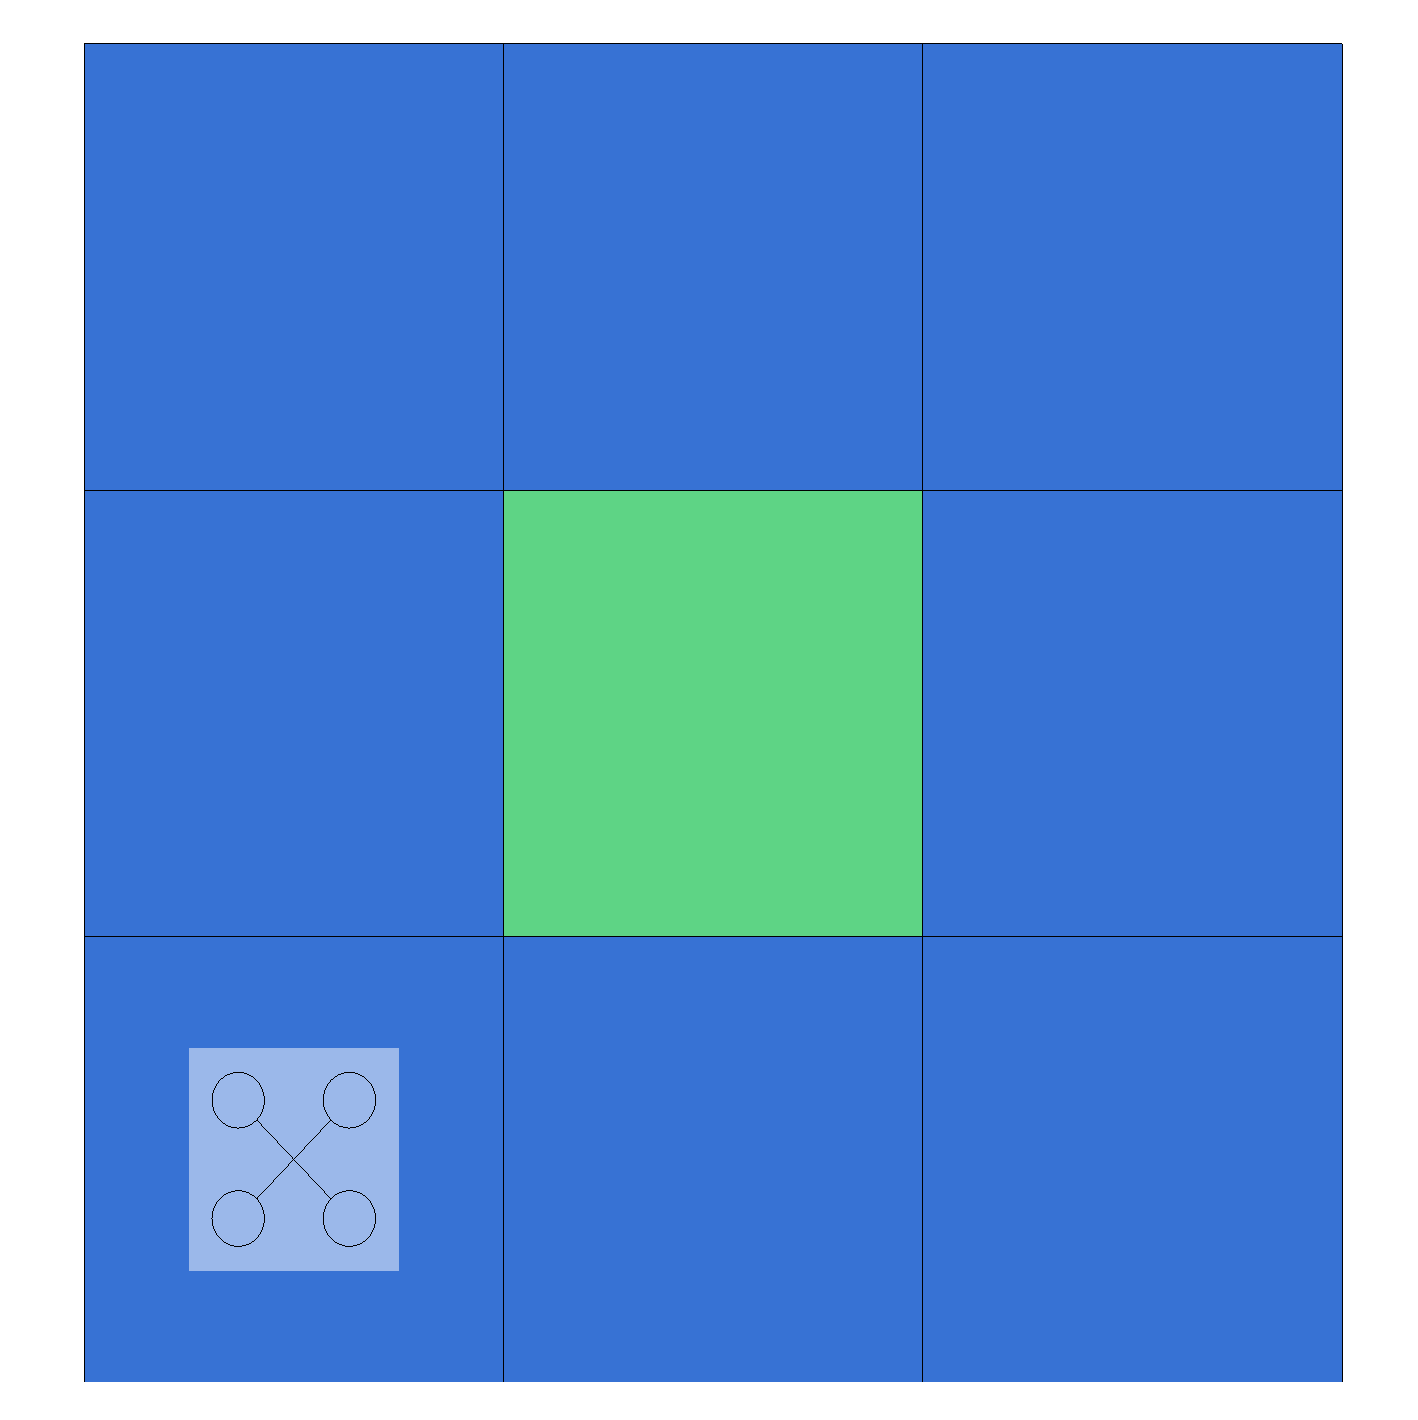
\includegraphics[width=\textwidth]{exampleEnv3Intro}
\caption[3x3 Env]{A very small environment with a drone at the lower left - this image is a placeholder.}
\end{figure}

Assume that a single drone must cover this environment starting from a low altitude over position (1,1). Because of this starting position, the drone immediately has access to the following information about the environment:




%recreate my wiki entry where I demonstrate a proof of concept for a distribution specific optimal strategy.

The above example makes it seem like the "High Sweep First" approach may be the best choice for a policy to complete this task. However, this is also not the case for all environments. Consider the following environment, for which the relative performance of the same two policies from last time is flipped:

%recreate the second environment from my wiki entry.

Both of these examples used very small environments in order to limit the length of explanations required. On this small a scale, the size and shape of the environment's Footprint provides a strong hint about the appropriate altitude switching strategy to employ when exploring the environment. Because the environment's Footprint is available to an agent before any decision needs to be made, it may be possible to create a policy that optimizes its behavior around that factor somewhat. However, for large environments that mostly consist of wide open space, the importance of this contribution on a case by case basis is likely to be minimal. Setting aside considerations about Footprint shape, the different ratios of High vs Low scrutiny patches used in these examples provide the first hint that the a priori unknown content of each environment has implications for the best possible strategy. As an extremely simple proof that this is the case, consider the following tiny environments:

%1: HL
%1: L 

%2: HH
%2: H

In both cases, assume that there is a single drone that starts at the top left position at a Low altitude.

In the first case, the best possible solution is to immediately Ascend. This action, whose move cost is as low or lower than all other move costs available in this simulation, completes the coverage task. Thus, this is clearly the optimal policy to use for exploring this environment in particular. In the second case, all environment cells require High scrutiny, and so must each be visited from a Low altitude. This means that the drone must move to each of the following states before the coverage tasks is complete:

\begin{enumerate}
	\item Low over Position (1, 1)
	\item Low over Position (0, 0)
\end{enumerate}

In this case, one optimal policy would be to move East and then South-West. This policy causes the scenario to complete in 24 time steps. More importantly, any Policy that starts out with an Ascend would then need to Descend before any of the necessary observations to complete coverage can be performed. These two altitude switching moves require a total of 20 time steps to complete, making it clearly impossible to finish the task in less than the 24 time steps that another policy demonstrates. With that, it has been demonstrated that a policy's chance at optimally exploring either of these environments can be ruined at the \textit{very first} move performed. The set of moves which keep a possibility of optimality in the first environment, {Ascend}, and the set of moves that do the same in the second environment, {MoveCardinal East, MoveCardinal South}, are disjoint. All of this is true despite the fact that policies operating in these two environments must make a decision based on precisely the same initial information:

%:?L?

This proves that it is impossible to create a policy that makes optimal decisions without assuming some distribution of possible environments. The exact degree to which environment distributions will affect policy performance on larger environments is not addressed analytically in this work. However, as later sections will demonstrate, experimental results show that this difference is quite dramatic.

As discussed in the previous chapter, oprc\_env is capable of generating quite a large number of different environments. Even if the exact parameters used by a particular environment generator are known in advance, it is not easy to characterize the distribution of resulting environments in a way that is useful for fine-tuning the design of policies. In addition, it seems intuitively likely that the distribution of real world environments in which this coverage behavior would be useful is similarly complex. This chapter will discuss the development and experimental optimization of Policy instances that do a good job on a complex distribution of environments.